\chapter{Hardware and Software Setup}

\section{Introduction}
In this section we will describe the principal components in terms of hardware and software and how they are interconnected to create a suitable robotic platform that will later be used for comparing the performance of \ac{LiDAR} and \ac{RADAR} as navigation sensors.  
\subsection{Turtlebot2}
TurtleBot 2 \fig{} is one of the  most popular low cost personal robots around. It is completely run by open source software which makes it exceptional for research and educational purposes. The robot has been developed by the Korean company Yujin Robotics in collaboration with Willow Garage, its differential kinematics mobile platform can be used for multiple applications, due to the huge number of available ROS packages.
The out of the box kobuki platform was modified in order to include a processing unit, a 2D scanning \ac{LiDAR} and a \ac{FMCW} radar as proximity sensors. The modified version is displayed in Fig.\ref{fig::turlebot2}. 
\begin{figure}[h] 
\centerline{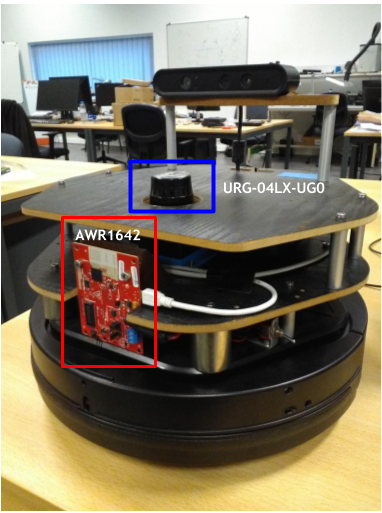
\includegraphics [width=0.3 \textwidth]{imgs/chapter4/turtlebot2.PNG}}
\caption{Modified Turtlebot2 used in this work}
\label{fig::turlebot2}
\end{figure}



\subsection{FMCW radar}

The radar board chosen for this work is the mmwave Texas Instruments AWR1642BOOST (Fig.\ref{fig:awr}). This is a recently distributed \ac{FMCW} radar dedicated for short range applications. The device supports a wide RF bandwidth of 77-81 GHz that permits good range and angle resolution.

\begin{figure}[h] 
\centerline{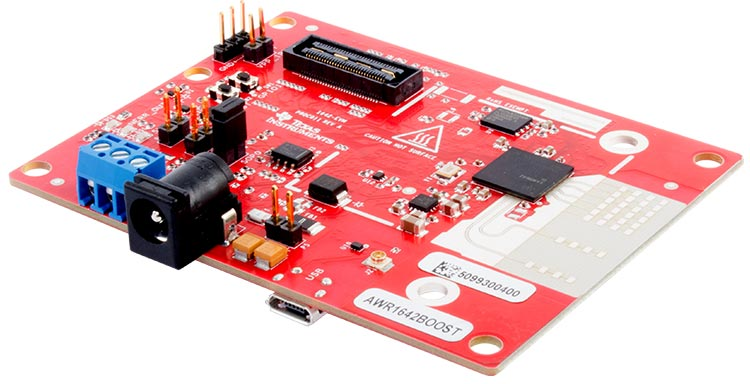
\includegraphics [width=0.5 \textwidth]{imgs/chapter4/awr1642.jpg}}
\caption{Texas Instruments AWR1642BOOST evaluation board}
\label{fig:awr}
\end{figure}

\subsection{LiDAR}
\begin{figure}[h] 
\centerline{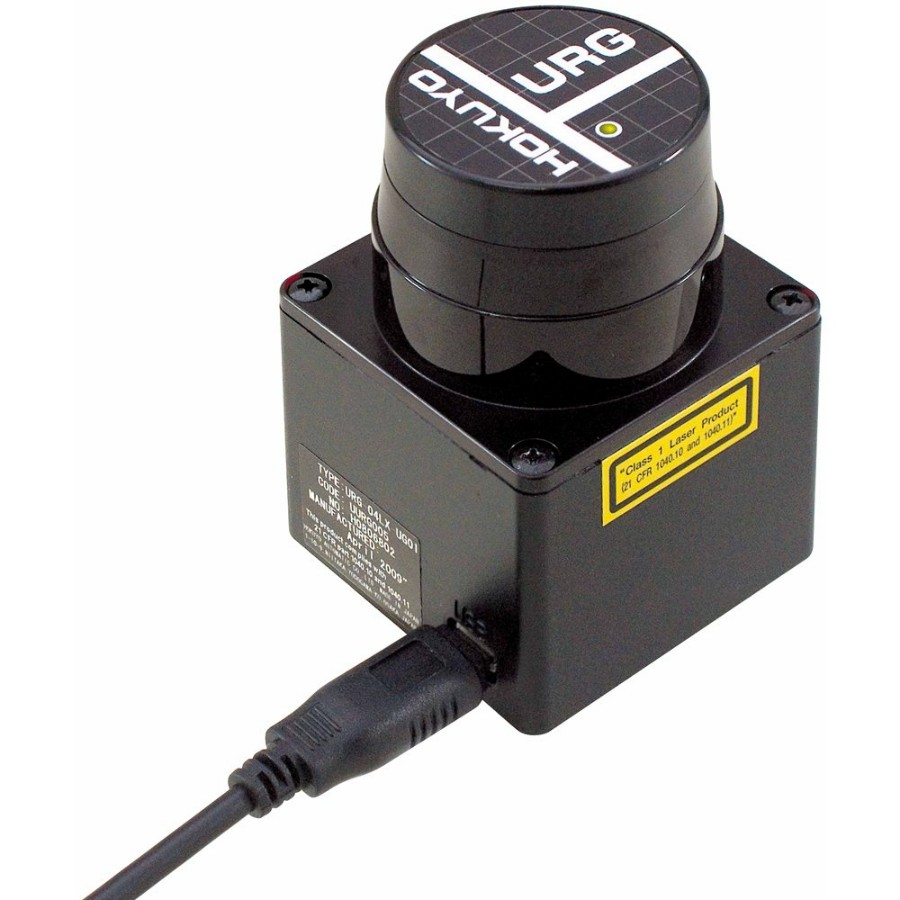
\includegraphics [width=0.5 \textwidth]{imgs/chapter4/lidar.jpg}}
\caption{lidar}
\label{fig:lidar}
\end{figure}

\section{Software Setup}

The software used in this project is divided in three stages. First one is the interface between the radar board TLV data and the ROS point cloud message format. Then using \ac{PCL} a filtering operation is added to remove false detections (this will be explained later). Finally, the filtered radar data as well as the \ac{LiDAR} data are fed to the ROS Navigation Stack as sensor sources. 
%%Block diagram

Figure X shows a simple block diagram describing   
\begin{figure}[h] 
\centerline{\includegraphics [width=0.3 \textwidth]{imgs/chapter5/blockdiagram.PNG}}
\caption{Modified Turtlebot2 used in this work}
\label{fig::turlebot2}
\end{figure}
\subsection{ROS radar driver}
Texas Instruments provides a ros package that interfaces radar data to the ROS message format \cite{tidriver}. The incoming radar TLV data from the mmWave EVM is decoded in order to create a  \textbf{PointCloud2} type ROS message.
This point cloud follows the detected objects frame described in the mmWave demo data structure \cite{}. 
Each point has 6 fields:
\begin{itemize}
\item \textbf{x (m)} - position x of the detected  object in the frame of the radar.
\item \textbf{y (m)} - position y.
\item \textbf{z (m)} - position z (for 2D devices this is equal to zero).
\item \textbf{range (m)} - range of the object relative to the radar frame.
\item \textbf{doppler (m/s)} - radial velocity of the object relative to the radar frame.
\item \textbf{intensity} - relative power of the received signal corresponding to that object.
\end{itemize}
\subsection{\ac{PCL} filtering}

\subsection{ROS Navigation stack}


\section{Summary}   

